\chapter{국소 양자장과 1차원 디랙 방정식}

양자장의 양자는 물론, 양자를 생성하고 소멸시키는 연산자와 비상대론적 입자의 가장 간단한 해밀토니안을 통해 양자장을 이미 살펴보았다. 이제 이 형식론을 실제로 활용해 보자. 먼저 공간적으로 국소적인 해밀토니안이 운동량을 보존한다는 사실을 단순히 주장하는 데 그치지 않고 직접 확인한다. 그런 다음 장의 곱으로 산란과 붕괴를 기술하고, 해밀토니안이 거듭 작용하면서 도식적 섭동론의 기본 형태가 어떻게 생겨나는지 살펴본다. 약속했던 페르미온 문제는 그 뒤에 다룬다. 가장 자연스러운 출발점은 아직 페르미온장이 아니라 1차원 디랙 방정식이다.

\section{장 해밀토니안을 다시 살펴보기}

비상대론적 입자 한 종의 해밀토니안을 다음과 같이 쓰자.
\begin{equation}
H_0=\int dx\,
\psi^\dagger(x)
\left[-\frac{\partial_x^2}{2m}+V(x)\right]
\psi(x).
\label{eq:l9-nonrel-hamiltonian}
\end{equation}
표기는 1차원처럼 보이지만, 도입부의 논의는 이 차원 제한에 의존하지 않는다. 3차원에서는 \(x\)를 벡터 \(\mathbf{x}\)로, \(dx\)을 \(d^3x\)로, \(-\partial_x^2\)를 \(-\nabla^2\)으로 바꾸면 된다.

연산자 \(\psi^\dagger(x)\)는 \(x\)에서 입자를 생성하고, \(\psi(x)\)는 그곳에서 입자를 소멸시킨다. 이들의 정상 순서 곱
\begin{equation}
n(x)=\psi^\dagger(x)\psi(x)
\end{equation}
은 국소 입자 수 밀도다. 따라서 퍼텐셜 항은 다음과 같이 쓸 수 있다.
\begin{equation}
H_V=\int dx\,V(x)n(x).
\end{equation}
이는 고전 기체에 대해 쓰는 식과 정확히 같다. \(x\) 근방의 입자 수를 세고, 각 입자에 퍼텐셜 에너지 \(V(x)\)를 부여한 뒤, 공간 전체에 걸쳐 더한다. 이 단계에서는 입자들이 서로 상호작용하지 않는다. 외부에서 가한 퍼텐셜에는 반응할 수 있지만, 그 외에는 해밀토니안이 서로 독립적인 일입자 에너지들의 합이다.

일단 단순화한 다음 다시 본래 문제로 돌아가는 편이 유용하다. 퍼텐셜을 상수 \(V(x)=V_0\)로 두자. 상수 퍼텐셜은 힘을 가하지 않지만, 연산자적 의미는 분명하다.
\begin{equation}
\begin{aligned}
H_V&=V_0\int dx\,\psi^\dagger(x)\psi(x)=V_0N,\\
N&=\int dx\,n(x).
\end{aligned}
\end{equation}
이는 각 입자에 같은 가산 에너지를 부여한다. 비상대론적 기술에서 정지 에너지를 포함하려면 \(V_0=mc^2\)로 택하면 된다. 그러면 이 항은 입자마다 정지 에너지 하나씩을 센다. 특별할 것 없는 이 상수항을 남겨 두는 이유는 병진 대칭을 보존하면서 입자 수를 세는 연산을 드러내기 때문이다.

\section{갱신 규칙으로서의 해밀토니안}

운동량이 보존된다는 말은 무슨 뜻일까? 해밀토니안이 하는 일을 중심으로 답해야 한다. \(\psi\)를 장 연산자, 일입자 파동함수, 다체 상태 모두를 나타내는 데 한꺼번에 쓰지 않도록, 다체 상태를 \(\lvert\Phi(t)\rangle\)라고 부르자. 짧은 시간 간격 \(\epsilon\) 동안에는
\begin{equation}
\lvert\Phi(t+\epsilon)\rangle
=\left(1-i\epsilon H+O(\epsilon^2)\right)
\lvert\Phi(t)\rangle,
\label{eq:l9-short-update}
\end{equation}
이며, 여기서 \(\hbar=1\)이다. 첫 번째 항은 변하지 않은 상태이고, 첫 번째 보정항은 \(H\)가 만들어 낸다. 이 갱신을 반복하면 Schr\"odinger 방정식이 나온다.

이제 운동량 보존의 의미가 구체적으로 드러난다. 초기 상태의 총운동량이 확정값 \(P\)을 가진다면, \(H\lvert\Phi\rangle\)도 같은 총운동량을 가져야 한다. 다른 성질은 변할 수 있고 개별 입자들은 서로 운동량을 주고받을 수도 있지만, 해밀토니안은 상태를 총 \(P\)이 다른 부분공간으로 옮길 수 없다. 해밀토니안을 운동량 기저로 다시 써서 이를 직접 확인할 수 있다.

\section{운동량 델타 함수로 나타나는 공간 적분}

푸리에 변환 규약을 다음과 같이 정하자.
\begin{align}
\psi(x)&=\int\frac{dp}{\sqrt{2\pi}}\,a(p)e^{ipx},\\
\psi^\dagger(x)&=\int\frac{dq}{\sqrt{2\pi}}\,a^\dagger(q)e^{-iqx}.
\label{eq:l9-field-fourier}
\end{align}
연산자 \(a(p)\)는 운동량 \(p\)인 입자를 소멸시킨다. 연산자 \(a^\dagger(q)\)는 운동량 \(q\)인 입자를 생성한다. 두 운동량은 공간 적분이 서로를 연결할 때까지 독립적으로 적분되므로, 서로 다른 문자를 쓰는 것이 중요하다.

수 항부터 시작하자.
\begin{align}
N
&=\int dx\,\psi^\dagger(x)\psi(x)\\
&=\int\frac{dp\,dq}{2\pi}\,
a^\dagger(q)a(p)
\int dx\,e^{i(p-q)x}.
\end{align}
남은 적분은
\begin{equation}
\int dx\,e^{i(p-q)x}=2\pi\delta(p-q).
\end{equation}
이다. \(p\ne q\)이면 위상이 진동하며 양의 기여와 음의 기여가 상쇄된다. \(p=q\)이면 전혀 진동하지 않는다. 디랙 델타 분포는 이 두 사실을 정확하게 결합하는 대상이다. 따라서
\begin{align}
N
&=\int dp\,dq\,a^\dagger(q)a(p)\delta(p-q)\\
&=\int dp\,a^\dagger(p)a(p).
\label{eq:l9-number-momentum}
\end{align}
이 연산자는 운동량 \(p\)인 입자를 제거하고 정확히 같은 운동량을 가진 입자를 다시 넣는다. 결정적인 역할을 한 것은 \(x\)에 대한 적분이었다. 이 적분으로 운동량의 입사값과 산출값이 같도록 하는 델타 함수가 생겼다.

\begin{classroomqa}\lecturetimestamp{00:17:02}\audiencequestion{\(p=q\)일 때 나타나는 무한대는 어떻게 된 건가요?}\lecturerresponse{델타 함수는 그 높이를 계산하는 방식으로 다루지 않는다. 델타 함수는 적분으로 정의되는 분포다. \(\int dk\,\delta(k)f(k)=f(0)\). ``무한히 높고 무한히 좁다''라는 표현은 적분된 가중치가 1임을 상기시킬 뿐이다. 여기서는 \(p-q=0\)으로 놓으라는 뜻이며, 따라서 무한한 답은 남지 않는다.}\end{classroomqa}

같은 원리는 훨씬 일반적인 국소 단항식에도 적용된다. 한 항에 소멸 장과 생성 장이 여러 개 포함되어 있고, 서로 다른 종에 속할 수도 있지만, 모두 한 점에서 평가되며 그 점에 대해 적분된다고 하자.
\begin{equation}
\int dx\,
\prod_{r=1}^{n} \psi_{i_r}^\dagger(x)
\prod_{s=1}^{m} \psi_{j_s}(x).
\end{equation}
소멸되는 입자들의 운동량을 \(p_s\), 생성되는 입자들의 운동량을 \(q_r\)라고 하자. 푸리에 전개를 대입하면
\begin{equation}
\int dx\,
e^{i(\sum_s p_s-\sum_r q_r)x}
=2\pi\,
\delta\!\left(\sum_s p_s-\sum_r q_r\right).
\label{eq:l9-total-momentum-delta}
\end{equation}
이 나온다. 이 결과는 \(p_1\)와 \(q_1\), \(p_2\)와 \(q_2\) 등을 각각 짝짓지 않는다. 결과가 부과하는 조건은 오직 다음뿐이다.
\begin{equation}
\sum_{\mathrm{annihilated}}p
=
\sum_{\mathrm{created}}q.
\end{equation}
이는 상호작용에 필요한 규칙과 정확히 일치한다. 개별 운동량은 변할 수 있지만 총운동량은 보존된다. 더 근본적인 진술은 병진 대칭성이다. 모든 점에 같은 가중치를 적용해 적분한 국소 밀도에는 특별한 원점이 없으며, 그 푸리에 변환에는 이에 대응하는 운동량 보존 델타 함수가 들어간다.

\begin{classroomqa}\lecturetimestamp{00:23:04}\audiencequestion{제안한 해밀토니안 항이 정말 저 장 연산자들을 모두 곱한 것인가요? 왜 그런 곱을 쓰나요?}\lecturerresponse{그렇다. 이 곱은 한 점에서 어떤 입자들을 제거하고 어떤 입자들을 생성하는지 명시한다. 그 물리적 동기는 관측된 산란이나 붕괴 과정에서 얻을 수 있다. 이 상호작용을 바로 읽어 낼 수 있도록 먼저 운동량에 관한 논의를 확립한 것이다.}\end{classroomqa}

\section{운동량 공간과 위치 공간에서의 운동 에너지}

이제 같은 형식론을 미분 항에 적용하자. 미분 연산자는 평면파에 작용한다.
\begin{equation}
-\partial_x^2 e^{ipx}=p^2e^{ipx}.
\end{equation}
따라서
\begin{align}
H_{\mathrm{kin}}
&=\int dx\,\psi^\dagger(x)
\left(-\frac{\partial_x^2}{2m}\right)\psi(x)\\
&=\int dp\,\frac{p^2}{2m}\,a^\dagger(p)a(p).
\label{eq:l9-kinetic-momentum}
\end{align}
를 얻는다. 여기서도 공간 적분은 입사 운동량과 산출 운동량이 같도록 한다. 새로 나타난 인자 \(p^2/2m\)는 각 운동량 모드의 입자 수에 해당 모드의 운동 에너지를 곱할 뿐이다.

\begin{classroomqa}\lecturetimestamp{00:24:46}\audiencequestion{평면파를 두 번 미분하면 마이너스 부호가 나와야 하지 않나요?}\lecturerresponse{그렇다. \(\partial_x^2e^{ipx}=-p^2e^{ipx}\). 해밀토니안에는 이를 상쇄하는 마이너스 부호가 이미 들어 있으므로, \(-\partial_x^2\)의 고유값은 양수인 \(p^2\)이다.}\end{classroomqa}

\begin{classroomqa}\lecturetimestamp{00:27:20}\audiencequestion{운동 에너지는 퍼텐셜이 상수일 때만 보존되나요?}\lecturerresponse{그렇다. 위치에 따라 변하는 퍼텐셜이 없으면 힘도 없으므로 운동 에너지는 별도로 보존된다. 위치에 따라 변하는 외부 퍼텐셜이 있으면 운동 에너지와 퍼텐셜 에너지가 서로 바뀔 수 있다. 다만 해밀토니안에 명시적인 시간 의존성이 없다면 전체 해밀토니안은 보존된다.}\end{classroomqa}

\begin{classroomqa}\lecturetimestamp{00:27:42}\audiencequestion{운동량 공간의 운동 해밀토니안에서 \(\psi^\dagger\psi\)는 어떤 역할을 하나요?}\lecturerresponse{입자 수를 세는 연산자다. 모드 곱 \(a^\dagger(p)a(p)\)은 운동량 \(p\)인 입자 수를 세고, 인자 \(p^2/2m\)는 각 입자에 해당 운동 에너지를 부여한다.}\end{classroomqa}

비음수성을 확인하는 두 번째 방법이 있다. 부분적분을 한 번 하고 경계항을 무시하면
\begin{align}
\int dx\,\psi^\dagger(-\partial_x^2)\psi
&=\int dx\,(\partial_x\psi^\dagger)(\partial_x\psi).
\label{eq:l9-positive-kinetic}
\end{align}
장이 무한대에서 적절히 영으로 가거나 주기적 경계조건을 만족하면 경계 기여분은 영이다. 결과는 절댓값의 제곱 꼴이므로 음이 아닌 값이다. 또한 장론에서 흔히 나타나는 양상, 즉 에너지에 장의 공간 미분의 제곱이 포함된다는 점도 보여 준다.

\section{국소 접촉 상호작용}

이제 장의 곱에 물리적 역할을 부여하자. 입자 종 두 가지를 생각하되, 익숙한 그림을 위해 전자와 양성자라고 부르겠다. 지금은 의도적으로 실제와 다르게 두 입자 모두 보손 연산자로 다루고, 실제 쿨롱 상호작용은 제외한다. 자유 해밀토니안은
\begin{equation}
H_0=\int dx\left[
\psi_e^\dagger\left(-\frac{\partial_x^2}{2m_e}\right)\psi_e
+
\psi_p^\dagger\left(-\frac{\partial_x^2}{2m_p}\right)\psi_p
\right].
\end{equation}
이다. 여기에 모형 상호작용을 더하자.
\begin{equation}
H_{\mathrm{contact}}
=g\int dx\,
\psi_e^\dagger(x)\psi_p^\dagger(x)
\psi_e(x)\psi_p(x).
\label{eq:l9-contact}
\end{equation}
오른쪽에서 왼쪽으로 읽어 보자. 한 점 \(x\)에서 전자와 양성자가 함께 있는지 확인하고, 이들을 소멸시킨 뒤 같은 점에서 둘 다 다시 생성한다. 두 입자가 함께 있지 않으면 이 국소 항은 0이다. 두 입자의 세계선이 만나면 개별 운동량은 바뀔 수 있지만 총운동량은 보존된다. 따라서 이 항은 이상화된 영거리 산란 퍼텐셜로 작용한다.

\begin{figure}[htbp]\centering
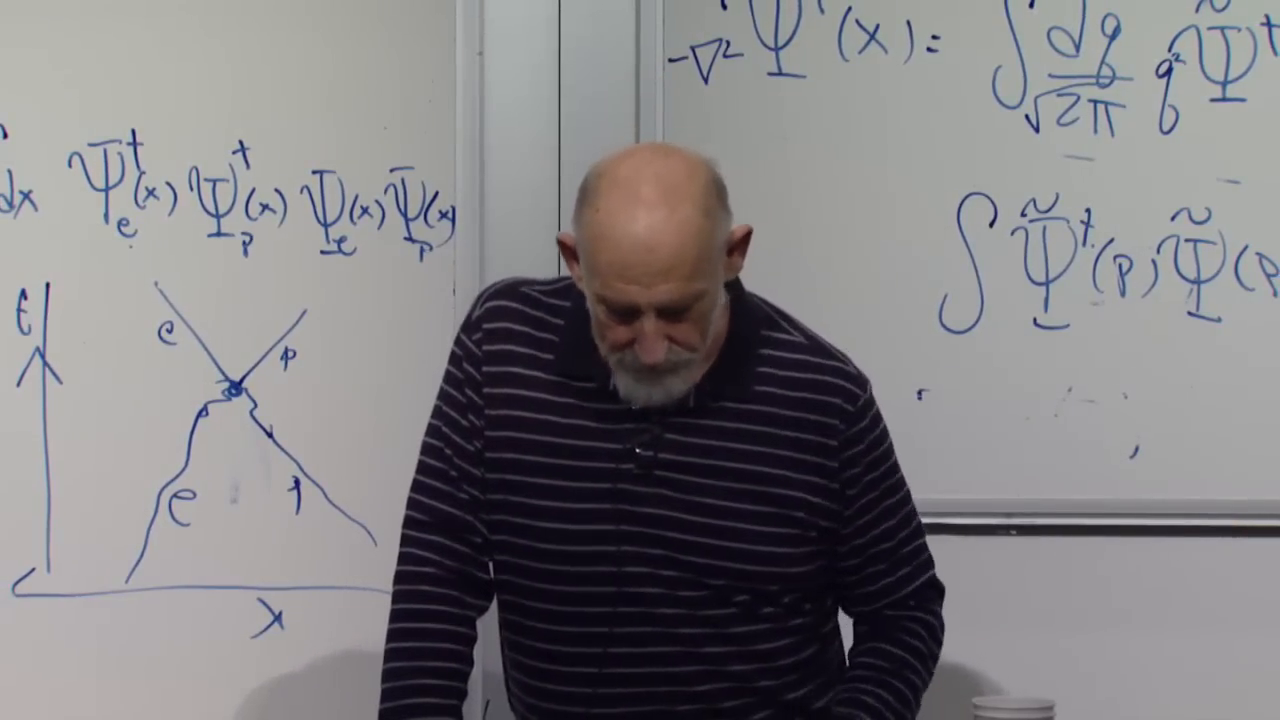
\includegraphics[width=0.94\linewidth]{lecture_09_frame_02.png}\caption{칠판의 접촉 상호작용. 네 개의 국소 장 연산자가 시공간 스케치 위에 나타나 있으며, 이상화된 상호작용은 만나는 점에서만 작용한다.}\lectureframe{00:35:36}\end{figure}

\begin{figure}[htbp]\centering
\begin{tikzpicture}[x=1.2cm,y=1.0cm,>=Latex]
\draw[->] (-3.0,0) -- (3.0,0) node[right] {$x$};
\draw[->] (0,-0.2) -- (0,4.2) node[above] {$t$};
\coordinate (v) at (0,2.0);
\fill (v) circle (1.8pt);
\draw[thick,->] (-2.2,0.4) -- (v);
\draw[thick,->] (2.0,0.4) -- (v);
\draw[thick,->] (v) -- (-1.6,3.7);
\draw[thick,->] (v) -- (2.2,3.7);
\node[left] at (-1.65,0.7) {$e$};
\node[right] at (1.55,0.7) {$p$};
\node[left] at (-1.15,3.3) {$e$};
\node[right] at (1.65,3.3) {$p$};
\node[right] at (0.12,2.05) {$g$};
\end{tikzpicture}\caption{국소 산란 그림을 깔끔하게 다시 그린 것이다. 꼭짓점은 식 ~\eqref{eq:l9-contact}의 연산자를 간략히 나타낸 것이며, 고전적인 충돌 법칙을 뜻하지 않는다.}\end{figure}

실제 전자와 양성자는 쿨롱 퍼텐셜을 통해 서로 떨어진 거리에서도 상호작용한다. 접촉 모형은 첫걸음일 뿐이다. 두 종이 서로 겹칠 때만 산란한다는 사실이 실험으로 밝혀진다면, 식 ~\eqref{eq:l9-contact}과 같은 항을 해밀토니안에 넣을 수 있다.

\begin{classroomqa}\lecturetimestamp{00:35:40}\audiencequestion{에너지가 변하지 않는데 왜 이 산란 연산자가 해밀토니안에 들어가나요?}\lecturerresponse{해밀토니안은 에너지 연산자인 동시에 상태를 변화시키는 생성자다. 두 입자 사이의 퍼텐셜 에너지는 시간발전에 따라 산란을 일으킨다. 전체 에너지가 보존된다고 해서 상태나 입자들의 개별 운동량까지 변하지 않는 것은 아니다.}\end{classroomqa}

이로부터 실용적인 규칙을 얻을 수 있다. 먼저 입자들이 어떤 국소 과정을 겪을 수 있는지 실험을 통해 알아낸다. 그런 다음 상태를 갱신하는 연산자에 그 과정을 부호화한다. 장의 곱은 장식적인 대수가 아니다. 대거가 붙은 인자와 붙지 않은 인자가 어떤 종의 입자가 나타나고 사라지는지를 지정한다.

\section{붕괴, 역과정, 에르미트성}

버블 챔버에서 종 \(A\)의 궤적이 한 점에서 끝나고, 그 점에서 종 \(B\)과 \(C\)의 궤적이 뻗어 나오는 것을 관측했다고 하자. 국소 과정은 다음과 같다.
\begin{equation}
A\longrightarrow B+C.
\end{equation}
이 과정을 일으키는 연산자는
\begin{equation}
V=g\int dx\,
\psi_B^\dagger(x)\psi_C^\dagger(x)\psi_A(x).
\label{eq:l9-decay-half}
\end{equation}
이다. 소멸 장은 \(A\)을 제거하고, 두 생성 장은 같은 점에서 \(B\)와 \(C\)를 만들어 낸다. 모든 \(x\)에 대해 같은 가중치로 적분하면 공간 병진 대칭성이 표현되고, 곧바로 다음 관계가 나온다.
\begin{equation}
p_A=p_B+p_C.
\end{equation}

해밀토니안은 에르미트 연산자여야 한다. 그래야 \(e^{-itH}\)가 유니터리이고 전체 확률이 보존된다. 식~\eqref{eq:l9-decay-half}만으로는 에르미트 연산자가 아니므로, 그 에르미트 수반을 더해야 한다.
\begin{equation}
H_{\mathrm{int}}
=\int dx\left[
g\,\psi_B^\dagger\psi_C^\dagger\psi_A
+g^*\,\psi_A^\dagger\psi_C\psi_B
\right](x).
\label{eq:l9-hermitian-vertex}
\end{equation}
결합 상수 \(g\)가 실수라면 두 계수는 같다. 에르미트 켤레를 취하면 대거의 유무를 서로 바꿀 뿐 아니라 연산자의 순서도 뒤집힌다. 이 보손 장난감 모형에서는 서로 다른 종의 장들이 교환하므로, 순서가 뒤집혀도 추가로 고려할 문제는 생기지 않는다.

두 번째 항은 역과정을 일으킨다.
\begin{equation}
B+C\longrightarrow A.
\end{equation}
따라서 붕괴를 허용하는 닫힌 유니터리 해밀토니안에는 재결합 진폭도 들어간다. 그렇다고 선택한 모든 외부 운동량 조건에서 두 방향의 과정이 모두 일어난다는 뜻은 아니다. 에너지 보존 등 다른 보존 법칙 때문에 한 방향의 과정이 운동학적으로 불가능할 수 있다. 이는 연산자와 그 수반이 모두 동역학에 포함된다는 뜻이다.

\begin{classroomqa}\lecturetimestamp{00:42:48}\audiencequestion{역과정도 허용되어야 한다는 규칙에 예외가 있을 수 있나요?}\lecturerresponse{에르미트성을 만족하는 닫힌 계의 해밀토니안에서는 그렇지 않다. 수반 상호작용이 반드시 필요하다. 특정 역반응은 운동학적 조건이나 다른 보존 양자수 때문에 여전히 금지될 수 있지만, 그 켤레 행렬 원소는 존재한다.}\end{classroomqa}

수 \(g\)은 결합 상수다. \(g\)가 작으면 만난 입자들은 약하게 상호작용하고, 크면 전이 진폭이 커진다. 결합 상수는 보통 실험으로 측정하는 매개변수지만, 대칭성에 의해 겉보기에 서로 달라 보이는 여러 결합 상수 사이의 관계가 정해질 수도 있다.

같은 문법으로 더 복잡한 반응도 다룰 수 있다. 베타 붕괴에서는
\begin{equation}
n\longrightarrow p+e^-+\bar\nu_e,
\end{equation}
중성자를 소멸시키고 양성자, 전자, 전자 반중성미자 세 입자를 생성하는 네 장의 도식적 국소 항과 그 에르미트 켤레 과정이 들어간다. 소수의 연산자 단항식으로 양자장론이 어떻게 구성되기 시작하는지 이를 통해 알 수 있다.

\section{해밀토니안의 제곱이 중요한 이유}

짧은 시간에 대한 식 \eqref{eq:l9-short-update}에서는 \(\epsilon\)의 일차항까지만 남겼다. 전체 전개는 다음과 같다.
\begin{equation}
e^{-i\epsilon H}
=1-i\epsilon H-\frac{\epsilon^2}{2}H^2
+\frac{i\epsilon^3}{3!}H^3+\cdots.
\label{eq:l9-exponential}
\end{equation}
이차항에서는 해밀토니안이 두 번 작용한다. 이것이 첫 복합 과정 그림이 생겨나는 대수적 기원이다.

상호작용 꼭짓점 \(A\leftrightarrow B+C\)의 경우, 한 번의 작용으로 \(B+C\)를 \(A\)로 합칠 수 있고, 두 번째 작용으로 그 \(A\)를 다시 \(B+C\)로 분해할 수 있다.
\begin{equation}
B+C\longrightarrow A\longrightarrow B+C.
\label{eq:l9-bc-scattering}
\end{equation}
그 결과로 \(B+C\to B+C\) 산란 진폭이 생긴다. 중간 상태 \(A\)는 별도로 관측되는 사건이 아니다. 두 번의 상호작용 작용 사이에서 합산되는 상태를 가리킨다.

\begin{classroomqa}\lecturetimestamp{00:49:54}\audiencequestion{기록된 2차 곱에서 \(C\) 장에는 대거가 붙어야 하지 않나요?}\lecturerresponse{그렇다. 연산자 순서는 서술된 과정의 순서와 일치해야 한다. 첫 번째 꼭짓점은 \(B\)과 \(C\)을 소멸시키고 \(A\)를 생성한다. 두 번째 꼭짓점은 \(A\)을 소멸시키고 \(B\)와 \(C\)를 다시 생성한다. 해당 연산자들에 대거를 올바르게 붙여 쓰면 이 해석과 일치한다.}\end{classroomqa}

\begin{figure}[htbp]\centering
\includegraphics[width=0.94\linewidth]{lecture_09_frame_05.png}\caption{칠판에 그린 기본 \(A\leftrightarrow B+C\) 꼭짓점의 두 방향. 두 그림을 나란히 놓으면 식 ~\eqref{eq:l9-bc-scattering}에 나타난 2차 과정을 간략하게 시각화할 수 있다.}\lectureframe{00:48:56}\end{figure}

이제 관전자 입자 \(B\)를 더하자. 한 번의 작용으로 \(A\)가 \(C\)를 방출해 \(B\)가 되고, 나중의 작용으로 그 \(C\)가 원래의 \(B\)와 결합해 \(A\)를 만든다. 외부 입자는 다시 \(A+B\)이지만, 운동량은 바뀔 수 있다. 이를 \(A\)와 \(B\)가 \(C\)를 교환하며 산란한다고 기술한다.

\begin{figure}[htbp]\centering
\includegraphics[width=0.94\linewidth]{lecture_09_frame_06.png}\caption{칠판에 그린 교환 과정. 오른쪽 그림은 두 기본 꼭짓점을 내부 \(C\) 선으로 연결하고, 외부 \(A\)와 \(B\) 입자가 산란하는 모습을 보여 준다.}\lectureframe{00:51:22}\end{figure}

\begin{figure}[htbp]\centering
\begin{tikzpicture}[x=1.1cm,y=1cm,>=Latex]
\draw[->] (-3.7,-0.2) -- (-3.7,4.2) node[above] {$t$};
\coordinate (v1) at (-0.9,1.25);
\coordinate (v2) at (0.9,2.95);
\fill (v1) circle (1.7pt);
\fill (v2) circle (1.7pt);
\draw[thick,->] (-2.6,0.2) -- (v1) node[midway,below left] {$A$};
\draw[thick,->] (2.6,0.2) -- (v2) node[midway,below right] {$B$};
\draw[thick,->] (v1) -- (-2.4,4.0) node[midway,left] {$B$};
\draw[thick,->] (v2) -- (2.5,4.0) node[midway,right] {$A$};
\draw[thick,->,dashed] (v1) -- (v2) node[midway,above left] {$C$};
\node[below] at (0,-0.05) {$A+B\rightarrow A+B$};
\end{tikzpicture}\caption{\(C\) 교환을 깔끔하게 다시 그린 그림이다. 각 점은 \(g\) 인자를 하나씩 주므로 이 2차 항은 \(g^2\)에 비례한다.}\end{figure}

각 국소 상호작용 점을 꼭짓점이라고 부른다. 각 꼭짓점은 해당 결합 상수의 인자를 하나씩 주므로, 꼭짓점 두 개가 있는 항에는 \(g^2\), 세 개가 있는 항에는 \(g^3\) 등이 들어간다. 따라서 해밀토니안의 항 하나가 여러 반응을 폭넓게 연관 짓는다. 소수의 국소 상호작용으로 방대한 산란 자료를 정리할 수 있다는 점이 양자장론이 강력한 이유 중 하나다.

\begin{classroomqa}\lecturetimestamp{00:53:14}\audiencequestion{과정 \(A\to B+C\to A\)는 무엇이라고 부르나요?}\lecturerresponse{자기에너지 기여다. 측정되는 \(A\)는 단지 맨입자 기저 상태인 것이 아니다. 상호작용하는 상태에는 가까운 \(B+C\) 성분을 가질 진폭도 있다. 산란을 통해 이런 드레싱된 구조를 알아낼 수 있다.}\end{classroomqa}

양자전기역학이 익숙한 예를 제공한다. 국소적인 전자--광자 꼭짓점은 전자를 소멸시키고, 전자를 다시 생성하며, 광자도 생성할 수 있다. 2차에서는 전자가 광자를 방출했다가 다시 흡수할 수 있다. 이를 작은 사건을 차례로 보여 주는 영화처럼 설명하고 싶어지지만, 엄밀한 의미에서 이는 섭동 전개의 한 항이다. 물리적 전자는 광자를 포함하는 성분을 가진 드레싱된 상태다.

이 성분이 ``약 1퍼센트''라는 수업 중의 추정은 미세구조 상수 \(\alpha_{\mathrm{em}}\simeq 1/137\)가 정하는 규모를 나타낸다. 광자 포크 성분의 정확한 확률은 에너지 분해능과 상호작용 상태의 정의에 달려 있다. 고립된 전자의 보편적인 1퍼센트 성질은 아니다. 확실하게 말할 수 있는 것은 상호작용이 전자의 측정 가능한 구조를 바꾼다는 점이다.

\section{도식이 말해 주는 것과 말해 주지 않는 것}

도식은 상호작용 해밀토니안의 거듭제곱을 계산하기 위한 간략한 표기다. 입자가 어떤 사건 하나를 확실히 겪은 다음 다른 사건을 겪는 고전적 이력으로 읽어서는 안 된다. 어떤 중간 대안이 ``실제로 일어났는지'' 알아보려 들면 실험이 달라지고, 보통의 양자 간섭에서와 마찬가지로 결맞은 합도 무너진다.

\begin{classroomqa}\lecturetimestamp{00:56:52}\audiencequestion{첫 번째 꼭짓점에서 에너지와 운동량이 모두 보존되나요?}\lecturerresponse{여기서 다룬 등시간 해밀토니안 구성에서는 공간 적분이 곧바로 운동량 델타 함수를 만든다. 이 삽입만으로는 시간 적분을 하지 않았으므로 에너지 델타 함수가 아직 생기지 않는다. 시간 병진 대칭인 전체 산란 진폭은 총에너지를 보존하지만, 중간선은 관측 입자에 적용되는 온셸 관계를 따르지 않아도 된다. 공변 도식 언어에서는 각 꼭짓점에서 사차원 운동량이 보존되지만, 내부 입자는 오프셸일 수 있다.}\end{classroomqa}

순진한 꼭짓점 그림에서 에너지가 사라진 것처럼 보이는 점은 상호작용 에너지를 무시해서는 안 된다는 또 하나의 경고다. 전체 해밀토니안은 자유 입자 에너지의 합보다 더 많은 것을 포함한다. 혼란스럽다면 식~\eqref{eq:l9-exponential}으로 돌아가자. 이 그림은 유니터리 시간발전 전개의 한 항을 나타낸다. 완전한 파인만 도식 형식론은 체계적인 시간 순서, 전파자, 적분, 대칭 인자를 제공하지만, 기본 물리는 여기서 시작된다.

한 가지 질문은 방출된 광자를 천천히 움직이는 전자를 둘러싼 전기장과 비교하며 도식을 지나치게 문자 그대로 해석한다.

\begin{classroomqa}\lecturetimestamp{00:58:26}\audiencequestion{전자에서 멀리 떨어진 곳의 전기장은 방출된 광자에 의해 문자 그대로 생기나요? 간섭과 아하로노프--봄 효과는 이 설명과 어떻게 양립하나요?}\lecturerresponse{정전기장이나 유도장은 실제 방출 광자의 흐름이 아니다. 양자전기역학은 복사와 전자의 전자기적 드레싱을 같은 장으로 기술하지만, 이에 대응하는 양자 상태와 운동학은 서로 다르다. 초상대론적 전자에서는 장의 일부 성분을 거의 실광자의 흐름으로 다루는 것이 유용할 수 있다. 느린 전자의 경우 광자가 문자 그대로 궤적을 따라간다는 모형은 맞지 않는다. 이중 슬릿 간섭과 아하로노프--봄 효과 역시 비고전적인 장 현상이지만, 그렇다고 자기에너지 도식을 역학적인 영화로 바꾸어 읽을 수 있는 것은 아니다.}\end{classroomqa}

\begin{classroomqa}\lecturetimestamp{01:01:28}\audiencequestion{도식의 고전적 모형이 정확히 왜 성립하지 않나요?}\lecturerresponse{계산에서 허용되는 모든 중간 대안의 진폭을 결맞게 더하기 때문이다. 익숙한 경험 덕분에 그림을 직관적으로 이해할 수는 있지만, 그림이 문자 그대로 뜻하는 바는 이를 정의하는 연산자 전개를 넘지 않는다. 그림은 \(H^2,H^3,\ldots\)을 계산하는 간결한 방법이지, 관측된 중간 사건의 기록이 아니다.}\end{classroomqa}

\begin{classroomqa}\lecturetimestamp{01:03:04}\audiencequestion{보통의 쿨롱 상호작용은 광자 교환의 고전적 극한으로 나타날 수 있나요?}\lecturerresponse{그렇다. 적절한 광자 매개 산란 진폭을 계산한 뒤 비상대론적 정적 극한을 취하면 쿨롱 퍼텐셜이 나온다. 이 유도는 지금 다루는 연산자 개요보다 기술적으로 복잡하며, 그래도 광자가 두 고전 입자 사이를 문자 그대로 오간다고 해석해서는 안 된다.}\end{classroomqa}

\begin{classroomqa}\lecturetimestamp{01:03:44}\audiencequestion{결합 상수는 장의 곱으로부터 계산하나요?}\lecturerresponse{대개 결합 상수의 수치는 실험으로 정한다. 대칭성은 결합 상수를 제약하거나, 그렇지 않으면 독립적일 여러 결합 상수 사이의 관계를 정할 수 있다. 그런 관계가 서로 다른 반응의 상대적 세기를 예측하고 실험으로 확인되면, 그 일치는 특히 많은 정보를 준다.}\end{classroomqa}

\begin{classroomqa}\lecturetimestamp{01:04:48}\audiencequestion{우연 대칭은 게이지 대칭과 어떤 점에서 다른가요?}\lecturerresponse{게이지 대칭은 허용되는 구조와 결합 상수 사이의 관계를 직접 제약한다. 우연 대칭은 근본 수준에서 부과된 것이 아니라, 허용되는 모든 낮은 차수의 상호작용이 우연히 그 대칭을 존중하기 때문에 나타난다. 우연 대칭도 중요한 결과를 낳을 수 있지만, 그 기원과 견고성은 게이지 대칭과 다르다.}\end{classroomqa}

비상대론적 장 이론은 일단 여기까지 살펴보자. 이제 페르미온을 다루기로 했다. 페르미온을 곧바로 제2양자화하는 대신, 먼저 페르미온의 장 연산자가 만족해야 하는 상대론적 일입자 방정식을 이해하자.

\section{전자에 상대론이 필요한 이유}

한 공간 차원에서 시작하자. 현실적인 제한은 아니지만, 3차원 스핀의 기하학적 복잡성을 덜어 내면서 핵심적인 대수 구조는 그대로 보존한다. 전자는 원자 안에서도 상대론을 고려해야 할 만큼 가볍다. 수소 원자에서 전자의 대표적인 속도는
\begin{equation}
v\sim\alpha_{\mathrm{em}}c\approx 0.007c,
\end{equation}
빛의 속도의 대략 1퍼센트다. 무거운 원자의 안쪽 전자에서는 대략적인 규모가 \(v\sim Z\alpha_{\mathrm{em}}c\)가 되어 상대론적 보정이 상당할 수 있다. 역사적 호기심에서 비롯된 동기든 원자 계산의 정확성에서 비롯된 동기든, 물리적으로는 상대론적 Schr\"odinger형 방정식이 필요하다.

통상적인 양자화 처방은 에너지와 운동량 사이의 고전적 관계에서 시작한다. 비상대론적 경우에는
\begin{equation}
E=\frac{p^2}{2m},
\end{equation}
이며, 다음 치환을 적용하면
\begin{equation}
E\mapsto i\partial_t,
\qquad
p\mapsto-i\partial_x
\end{equation}
다음 방정식을 얻는다.
\begin{equation}
i\partial_t\varphi(x,t)
=-\frac{1}{2m}\partial_x^2\varphi(x,t).
\end{equation}

상대론에서는 \(c=1\)로 두면 다음 관계가 성립한다.
\begin{equation}
E^2=p^2+m^2.
\label{eq:l9-rel-dispersion}
\end{equation}

\begin{figure}[htbp]\centering
\includegraphics[width=0.94\linewidth]{lecture_09_frame_07.png}\caption{칠판에서 \(E=p^2/2m\)에서 상대론적 관계 \(E^2=p^2+m^2\)로 넘어간다. 여기서는 \(c=1\)이다.}\lectureframe{01:10:30}\end{figure}

제곱된 관계식에 치환을 적용하면
\begin{equation}
-\partial_t^2\varphi
=\left(-\partial_x^2+m^2\right)\varphi,
\label{eq:l9-klein-gordon}
\end{equation}
을 얻는다. 이를 다음과 같이 쓸 수도 있다.
\begin{equation}
\left(\partial_t^2-\partial_x^2+m^2\right)\varphi=0.
\end{equation}
이것이 클라인--고든 방정식이다. 특히 스핀이 0인 장에 대해 충분히 의미 있는 상대론적 장 방정식이다. 하지만 전자에 필요한 방정식은 시간에 대해 1차여야 한다.
\begin{equation}
i\partial_t\Psi=H\Psi,
\end{equation}
그래야 \(H\) 자체가 시간발전을 생성하고, \(H^2\)만으로 그 역할을 하지 않는다.

형식적으로 다음과 같이 정할 수도 있다.
\begin{equation}
H=\sqrt{-\partial_x^2+m^2}.
\end{equation}
운동량 공간에서는 제곱근이 \(\sqrt{p^2+m^2}\)을 곱하는 방식으로 명확히 정의되지만, 위치 공간에서는 비국소적인 유사 미분 연산자다. 수학적으로는 의미가 있지만 우리가 원하는 국소 방정식에는 미적으로 적합하지 않다. 따라서 처음부터 다시 시작하자.

\section{질량이 없는 우향 진행파}

먼저 오른쪽으로 움직이는 질량 없는 입자를 생각하자. 양의 에너지와 운동량은 다음 관계를 만족한다.
\begin{equation}
E=p
\qquad (c=1).
\end{equation}
양자화하면
\begin{equation}
i\partial_t\psi=-i\partial_x\psi,
\end{equation}
또는
\begin{equation}
(\partial_t+\partial_x)\psi=0.
\label{eq:l9-right-mover}
\end{equation}
을 얻는다. 모든 해는 다음 형태다.
\begin{equation}
\psi(x,t)=f(x-t).
\end{equation}
파형의 모양은 변하지 않은 채 빛의 속도로 오른쪽으로 움직인다.

두 가지 문제가 즉시 드러난다. 첫째, 식 ~\eqref{eq:l9-right-mover}이 임의의 푸리에 모드에 작용하도록 허용하면, 음의 운동량의 에너지는 \(E=p<0\)가 되어 해밀토니안에 하한이 없다. \(p>0\)로 제한하면 오른쪽으로 진행하는 모드만 남지만, 이것만으로는 우리가 원하는 전자 이론이 되지 않는다. 둘째, 이 방정식은 한쪽 방향만 허용해 보통의 왼쪽 진행 전자가 들어 있지 않다. 먼저 좌우 방향의 문제를 해결하고 음의 에너지는 드러난 채로 두자.

\section{두 성분과 알파 행렬}

진폭 두 개를 도입하자.
\begin{equation}
\Psi(x,t)=
\begin{pmatrix}
\psi_1(x,t)\\[3pt]
\psi_2(x,t)
\end{pmatrix},
\end{equation}
여기서 질량이 없는 극한에 \(\psi_1\)는 오른쪽으로, \(\psi_2\)는 왼쪽으로 진행한다.
\begin{align}
(\partial_t+\partial_x)\psi_1&=0,
&
(\partial_t-\partial_x)\psi_2&=0.
\end{align}
양자역학에서는 둘의 임의의 중첩도 가능하다. 따라서 입자는 고전적인 꼬리표 하나를 처음부터 끝까지 지니는 대신, 양쪽 진행 방향 모두에 대한 진폭을 가질 수 있다.

이 추가적인 2값 자유도는 대수적으로 스핀과 비슷하지만, 1차원에서는 통상적인 각운동량이 아니다. 다음과 같이 정의하자.
\begin{equation}
\alpha=
\begin{pmatrix}
1&0\\
0&-1
\end{pmatrix}
=\sigma_3.
\label{eq:l9-alpha}
\end{equation}
그 \(+1\) 고유벡터는 오른쪽으로 진행하는 성분을, \(-1\) 고유벡터는 왼쪽으로 진행하는 성분을 선택한다. 질량이 없는 이론에서 해밀토니안은 단순히
\begin{equation}
H=\alpha p,
\end{equation}
이고, 두 방정식을 합치면
\begin{equation}
i\partial_t\Psi=-i\alpha\partial_x\Psi.
\label{eq:l9-massless-dirac}
\end{equation}

\begin{classroomqa}
\lecturetimestamp{01:22:44}
\audiencequestion{두 성분을 구별하는 대각행렬의 이름은 무엇인가요?}
\lecturerresponse{파울리 행렬로는 \(\sigma_3\)이며, \(\sigma_1\)은 아닙니다. 여기서 구성한 디랙 표기법에서는 이를 \(\alpha\)라고 부릅니다. 여기서 물리적으로 나타내는 것이 스핀 각운동량이 아니라 방향이지만, 그 대수는 익숙한 파울리 대수와 같습니다.}
\end{classroomqa}

\begin{classroomqa}
\lecturetimestamp{01:23:32}
\audiencequestion{방향이 벡터인 3차원에서는 이 구성이 더 기하학적인 의미를 갖나요?}
\lecturerresponse{그렇습니다. 3차원 문제에서는 공간의 각 방향에 대응하는 행렬이 하나씩 필요하며, 더 풍부한 스피너 구조가 나타납니다. 그래도 1차원 모형은 그 자체의 조건에서 정확하며, 추가적인 복잡성 없이 핵심적인 좌우 대수를 분리해 보여 줍니다.}
\end{classroomqa}

\begin{figure}[htbp]
\centering
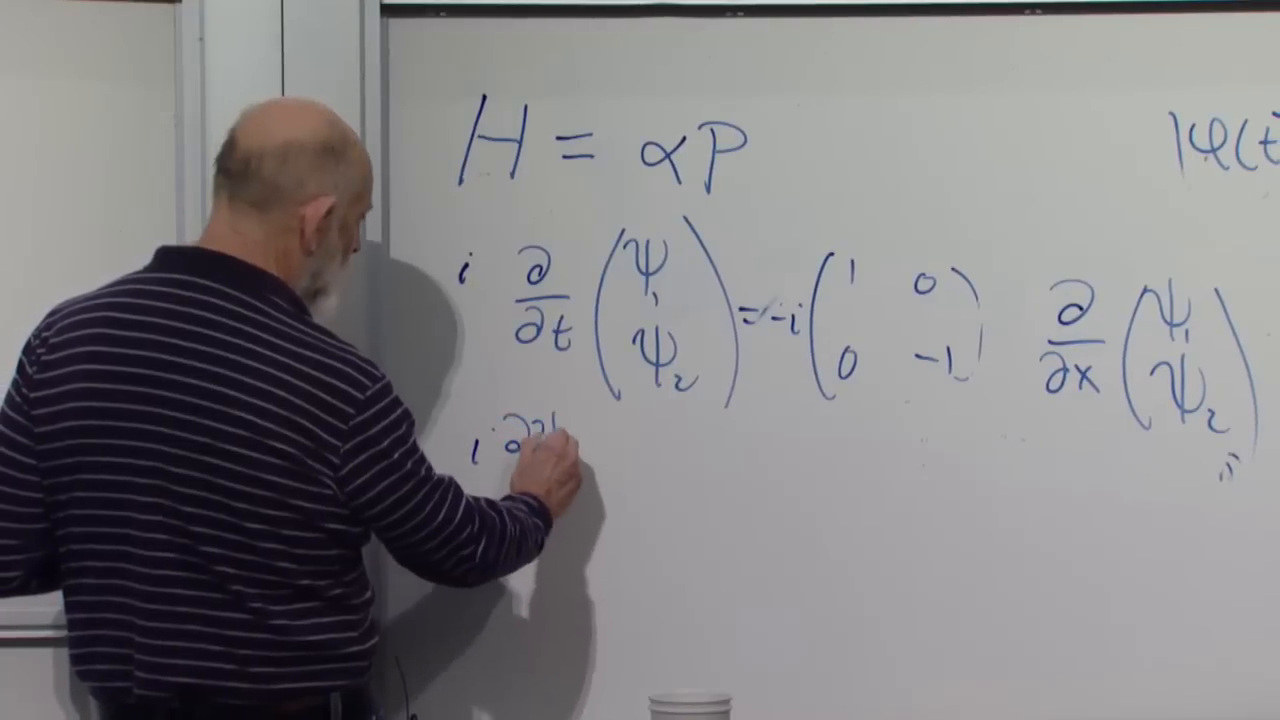
\includegraphics[width=0.94\linewidth]{lecture_09_frame_03.png}
\caption{칠판에 적힌 질량 없는 2성분 방정식: \(H=\alpha P\)에서 대각행렬은 \(\psi_1\)와 \(\psi_2\)에 서로 반대 방향의 전파를 부여한다.}
\lectureframe{01:26:00}
\end{figure}

한쪽 방향으로만 진행하는 문제는 해결되었다. 음에너지 스펙트럼은 여전히 남아 있고, 세 번째 결함도 드러났다. 두 성분이 여전히 질량이 없으며 빛의 속도로 전파된다는 점이다. 다음 단계에서는 정지에너지를 도입하고 두 방향을 결합해야 한다.

\section{질량을 더하고 디랙 대수를 발견하다}

질량에 비례하는 가장 일반적인 간단한 항을 더하자.
\begin{equation}
H=\alpha p+\beta m,
\label{eq:l9-dirac-hamiltonian}
\end{equation}
여기서 \(\beta\)은 2성분 지표에만 작용한다. 이 행렬은 항등행렬이나 다른 행렬일 수도 있다. 어떤 행렬을 택할지는 상대론적 분산 관계에 맡기자.

\(H^2\)이 \(p^2+m^2\)와 같아야 하므로, 식~\eqref{eq:l9-dirac-hamiltonian}을 제곱하면
\begin{align}
H^2
&=(\alpha p+\beta m)^2\\
&=\alpha^2p^2+\beta^2m^2
+(\alpha\beta+\beta\alpha)pm.
\label{eq:l9-square-dirac}
\end{align}
행렬들은 내부의 2성분 공간에 작용하고 \(p\)는 공간 파동함수에 작용하므로, 이 행렬들은 \(p\)와 가환한다. 식~\eqref{eq:l9-rel-dispersion}에 맞추려면 다음 조건이 필요하다.
\begin{equation}
\alpha^2=\mathbb{1},
\qquad
\beta^2=\mathbb{1},
\qquad
\{\alpha,\beta\}
=\alpha\beta+\beta\alpha=0.
\label{eq:l9-dirac-algebra}
\end{equation}
첫 번째 조건은 이미 \(\alpha=\sigma_3\)에 대해 성립한다. 다른 파울리 행렬은 어느 것이든 이것과 반가환하며 제곱하면 항등행렬이 된다. 다음을 택하자.
\begin{equation}
\beta=
\begin{pmatrix}
0&1\\
1&0
\end{pmatrix}
=\sigma_1.
\label{eq:l9-beta}
\end{equation}
\(\sigma_2\) 대신 \(\sigma_1\)을 택한 것은 기저에 관한 관례일 뿐이다. 유니터리 기저 변환을 하면 두 선택은 같은 대수를 나타낸다.

\begin{classroomqa}
\lecturetimestamp{01:33:00}
\audiencequestion{디랙은 이 대수 조건을 만족하는 것이 파울리 행렬임을 그저 알아차린 건가요?}
\lecturerresponse{역사적으로는 3차원에서 직접 유도하여 필요한 관계를 만족하는 행렬들을 도입했습니다. 조건을 써 놓고 나면, 파울리 대수 덕분에 1차원 해는 즉시 얻을 수 있습니다. 서로 다른 파울리 행렬 두 개를 택하면 됩니다.}
\end{classroomqa}

\begin{classroomqa}
\lecturetimestamp{01:34:24}
\audiencequestion{이 \(\beta\)는 상대론적 속도 매개변수 \(v/c\)인가요?}
\lecturerresponse{아닙니다. 스피너 성분에 작용하는 행렬입니다. 같은 문자를 쓴 것은 디랙의 표기법일 뿐이며, 운동학적 양인 \(v/c\)와는 아무 관계가 없습니다.}
\end{classroomqa}

3차원 공간에서는 필요한 반가환 행렬 전체를 구성하기에 \(2\times2\) 행렬만으로는 충분하지 않다. 행렬을 확장하는 일은 뒤로 미룬다. 1차원에서는 식~\eqref{eq:l9-alpha}과 \eqref{eq:l9-beta}이면 충분하다.

\section{1차원 결합 디랙 방정식}

\(p=-i\partial_x\)를 대입하면 해밀토니안 형식의 1차원 디랙 방정식을 얻는다.
\begin{equation}
i\partial_t\Psi
=\left(-i\alpha\partial_x+\beta m\right)\Psi.
\label{eq:l9-one-dimensional-dirac}
\end{equation}
\(\alpha\)은 대각행렬이므로 미분항은 두 성분을 서로 분리해 둔다. \(\beta\)는 비대각행렬이므로 질량항은 두 성분을 서로 바꾼다. 성분별로 쓰면
\begin{align}
i\partial_t\psi_1
&=-i\partial_x\psi_1+m\psi_2,
\label{eq:l9-dirac-component-one}\\
i\partial_t\psi_2
&=+i\partial_x\psi_2+m\psi_1.
\label{eq:l9-dirac-component-two}
\end{align}

\begin{figure}[htbp]
\centering
\includegraphics[width=0.94\linewidth]{lecture_09_frame_08.png}
\caption{칠판에 적힌 결합 성분 방정식. 미분항의 부호가 서로 반대인 것은 오른쪽 및 왼쪽 방향의 운동을 나타내고, 비대각 질량항은 \(\psi_1\)와 \(\psi_2\)를 서로 바꾼다.}
\lectureframe{01:37:44}
\end{figure}

\(m\ne0\)이면 성분들은 더 이상 서로 독립적으로 진화하지 않는다. 1차 방정식을 제곱하면 각 성분에 대해 클라인--고든 연산자를 다시 얻는다,
\begin{equation}
\left(\partial_t^2-\partial_x^2+m^2\right)\psi_a=0,
\qquad a=1,2,
\end{equation}
그리고 평면파는 \(E^2=p^2+m^2\)을 만족한다. 군속도는
\begin{equation}
v_g=\frac{dE}{dp}=\frac{p}{E},
\end{equation}
이며, 질량이 영이 아니면 그 크기는 하나보다 작다.

질량과 좌우 성분의 혼합 사이의 관계는 우연이 아니다. 질량이 없는 오른쪽 진행 입자는 모든 적절한 로런츠 부스트 아래에서도 오른쪽으로 계속 진행한다. 빛보다 빠르게 앞질러 그 방향을 뒤집을 수 있는 아광속 관측자는 없기 때문이다. 질량이 있는 입자는 정지 상태로 만들 수 있고, 이어서 같은 방향으로 더 빠르게 움직이는 좌표계에서 관측할 수 있다. 이 좌표계에서는 입자의 속도가 반대 방향으로 보인다. 따라서 질량이 있는 상대론적 이론에서 오른쪽 및 왼쪽 부문을 영구히 분리해 둘 수는 없다. 비대각 질량항이 바로 필요한 결합을 제공한다.

\begin{classroomqa}
\lecturetimestamp{01:40:01}
\audiencequestion{두 성분이 서로 바뀌는 것을 키랄 진동이라고 하나요?}
\lecturerresponse{이 1차원 기저에서 \(\alpha\)는 질량이 없는 두 키랄 방향을 구별합니다. 질량항은 비대각이어서 두 방향을 혼합하므로 키랄성은 더 이상 보존되지 않습니다. 그런 의미에서 질량항이 키랄 진동의 원인입니다.}
\end{classroomqa}

\begin{classroomqa}
\lecturetimestamp{01:40:46}
\audiencequestion{페르미온 방정식이 왜 보손 방정식의 제곱근이어야 하나요?}
\lecturerresponse{그렇게 이해해서는 안 됩니다. 분산 관계 \(E^2=p^2+m^2\)는 통계적 성질과 관계없이 모든 자유 상대론적 입자에 적용됩니다. 디랙 연산자가 클라인--고든 연산자의 행렬 인수분해를 제공하기는 하지만, 이 대수적 관계가 보손으로부터 페르미온을 유도하는 것은 아닙니다.}
\end{classroomqa}

\begin{classroomqa}
\lecturetimestamp{01:41:31}
\audiencequestion{방정식을 왼쪽 및 오른쪽으로 진행하는 인수들로 이루어진 간단한 스칼라 인수분해로 바꿀 수 있나요?}
\lecturerresponse{질량이 없는 극한에서만 두 키랄 방정식이 서로 분리된 스칼라 인수들로 분리됩니다. \(m\ne0\)일 때 유용한 인수분해는 행렬을 사용하는 방식입니다. 원치 않는 교차항을 없애 주는 것은 서로 반가환하는 \(\alpha\)와 \(\beta\) 행렬입니다.}
\end{classroomqa}

\begin{classroomqa}
\lecturetimestamp{01:42:04}
\audiencequestion{이 결합된 두 방정식이 이미 디랙 방정식인가요?}
\lecturerresponse{그렇습니다. 두 방정식을 함께 쓰면 1차원 공간에서의 디랙 방정식이며, 식~\eqref{eq:l9-one-dimensional-dirac}의 간결한 형식과 같습니다. \(\beta\)를 곱하면 더 대칭적인 공변 표기를 얻을 수 있지만, 그 형식은 뒤에서 다룹니다.}
\end{classroomqa}

일부러 아직 마무리하지 않은 과제가 두 가지 남아 있다. 이 구성은 음에너지를 없애지 않았다. 두 방향 부문 모두에 음에너지 해를 제공했으므로, 이 문제는 해결되기는커녕 이제 더 분명해졌다. 또한 이 이론은 여전히 한 공간 차원에 놓여 있다. 음에너지 해를 해석하고 행렬 대수를 \(3+1\)차원으로 확장하는 것이 다음 단계다.
